\documentclass[11pt,a4paper]{article}
\usepackage[margin=1in]{geometry}
\usepackage{booktabs}
\usepackage{listings}
\usepackage{xcolor}
\usepackage{hyperref}
\usepackage{amsmath}
\usepackage{tikz}
\usetikzlibrary{arrows.meta}

\lstset{
  basicstyle=\ttfamily\small,
  breaklines=true,
  frame=single,
  language=Python,
  keywordstyle=\color{blue},
  commentstyle=\color{gray}\itshape,
  showstringspaces=false
}

\title{DM--J4310--2EC V1.1 -- Motor Notes\\
\large Communication, Control Modes, Code Audit}
\author{}
\date{}

\begin{document}
\maketitle

% =========================================================================
\section{Motor Calibration -- Setup and Verification}
\label{sec:calibration}
% =========================================================================

Correct operation requires three calibration layers applied in order.
An error in any layer is the most common source of ``wrong position'',
``motor does not move'', or ``feedback always zero''.

% ---- Overview: three-layer flowchart -------------------------------------
\subsection{The three calibration layers}

\begin{figure}[ht]
\centering
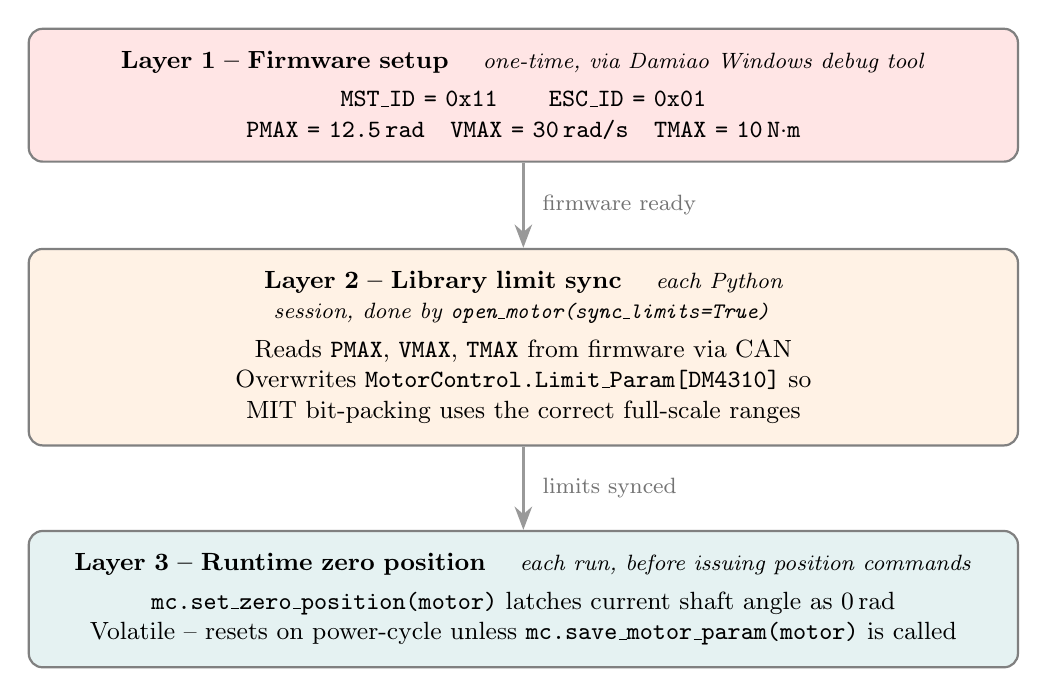
\begin{tikzpicture}[every node/.style={font=\small}]
  \node[draw=black!50, thick, rounded corners=5pt, fill=red!10,
        text width=12cm, minimum height=1.6cm, align=center, inner sep=8pt]
    (l1) at (0, 0) {
      \textbf{Layer~1 -- Firmware setup}
      \quad\textit{\footnotesize one-time, via Damiao Windows debug tool}\\[3pt]
      \texttt{MST\_ID = 0x11}\qquad \texttt{ESC\_ID = 0x01}\\
      \texttt{PMAX = 12.5\,rad}\quad \texttt{VMAX = 30\,rad/s}\quad
      \texttt{TMAX = 10\,N$\cdot$m}
  };
  \node[draw=black!50, thick, rounded corners=5pt, fill=orange!10,
        text width=12cm, minimum height=1.6cm, align=center, inner sep=8pt]
    (l2) at (0, -3.2) {
      \textbf{Layer~2 -- Library limit sync}
      \quad\textit{\footnotesize each Python session, done by
      \texttt{open\_motor(sync\_limits=True)}}\\[3pt]
      Reads \texttt{PMAX}, \texttt{VMAX}, \texttt{TMAX} from firmware via CAN\\
      Overwrites \texttt{MotorControl.Limit\_Param[DM4310]} so MIT
      bit-packing uses the correct full-scale ranges
  };
  \node[draw=black!50, thick, rounded corners=5pt, fill=teal!10,
        text width=12cm, minimum height=1.6cm, align=center, inner sep=8pt]
    (l3) at (0, -6.4) {
      \textbf{Layer~3 -- Runtime zero position}
      \quad\textit{\footnotesize each run, before issuing position commands}\\[3pt]
      \texttt{mc.set\_zero\_position(motor)} latches current shaft angle
      as $0\,\mathrm{rad}$\\
      Volatile -- resets on power-cycle unless
      \texttt{mc.save\_motor\_param(motor)} is called
  };
  \draw[-Stealth, thick, black!40, line width=1.2pt]
    (l1.south) -- node[right, font=\footnotesize, xshift=3pt, text=black!55]
    {firmware ready} (l2.north);
  \draw[-Stealth, thick, black!40, line width=1.2pt]
    (l2.south) -- node[right, font=\footnotesize, xshift=3pt, text=black!55]
    {limits synced} (l3.north);
\end{tikzpicture}
\caption{Three calibration layers required before commanding the motor.
         All three must be correct; each layer depends on the one above it.}
\label{fig:calib-layers}
\end{figure}

% ---- Layer 1 -------------------------------------------------------------
\subsection{Layer~1: Firmware parameter setup}

Use the \textbf{Damiao Windows debug tool} connected via USB (Write Param tab):

\begin{center}\small
\begin{tabular}{llll}
\toprule
Parameter & Required value & Effect if wrong & How to fix\\
\midrule
\texttt{MST\_ID} & \textbf{0x11} (not \texttt{0x00}!) &
  All feedback dropped; \texttt{getPosition()} returns 0 &
  Write Param\\
\texttt{ESC\_ID} & \texttt{0x01} (default) &
  Python driver cannot address motor &
  Write Param\\
\texttt{PMAX} & 12.5\,rad &
  Position commands silently rescaled &
  Verify/adjust\\
\texttt{VMAX} & 30\,rad/s &
  Velocity commands silently rescaled &
  Verify/adjust\\
\texttt{TMAX} & 10\,N$\cdot$m &
  Torque commands silently rescaled &
  Verify/adjust\\
\bottomrule
\end{tabular}
\end{center}

\noindent Dump all current firmware values:
\begin{lstlisting}
python tests/damiao/01_read_params.py
\end{lstlisting}

\noindent Fix \texttt{MST\_ID} via Python if the debug tool is unavailable:
\begin{lstlisting}
# tests/damiao/02_write_params.py -- set at top, run once
PARAM   = DM_variable.MST_ID
VALUE   = 0x11
PERSIST = True   # calls save_motor_param() to survive power cycle
\end{lstlisting}

\subsubsection*{Why \texttt{MST\_ID = 0x11} is critical}

The motor embeds its \texttt{MST\_ID} as the CAN~ID of every feedback
frame.  The Python driver accepts only frames whose CAN~ID matches the
\texttt{MasterID} argument passed to \texttt{Motor(\ldots, MasterID=0x11)}.

\begin{figure}[ht]
\centering
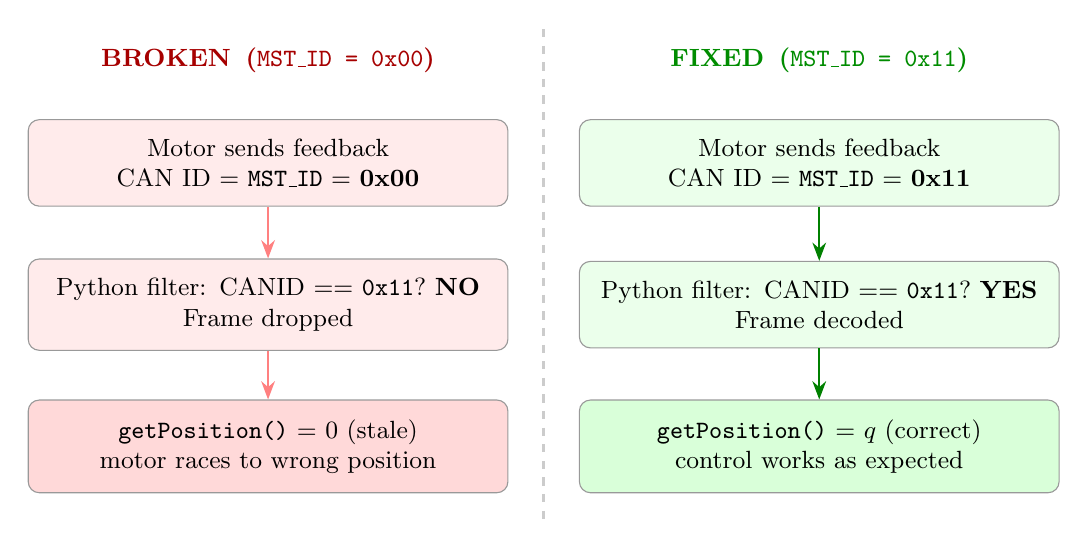
\begin{tikzpicture}[every node/.style={font=\small},
  cbox/.style={draw=black!40, rounded corners=4pt, inner sep=7pt,
               text width=5.6cm, align=center, minimum height=0.9cm}]

  \node[font=\small\bfseries, text=red!65!black]
    at (-3.5, 1.9) {BROKEN\enspace(\texttt{MST\_ID = 0x00})};
  \node[font=\small\bfseries, text=green!55!black]
    at ( 3.5, 1.9) {FIXED\enspace(\texttt{MST\_ID = 0x11})};
  \draw[dashed, black!20, line width=1pt] (0, 2.3) -- (0, -4.0);

  % Broken path
  \node[cbox, fill=red!8]  (bm) at (-3.5,  0.6)
    {Motor sends feedback\\CAN~ID = \texttt{MST\_ID} = \textbf{0x00}};
  \node[cbox, fill=red!8]  (bf) at (-3.5, -1.2)
    {Python filter: CANID~==~\texttt{0x11}?~\textbf{NO}\\Frame dropped};
  \node[cbox, fill=red!15] (br) at (-3.5, -3.0)
    {\texttt{getPosition()} = 0 (stale)\\motor races to wrong position};
  \draw[-Stealth, red!50, thick] (bm) -- (bf);
  \draw[-Stealth, red!50, thick] (bf) -- (br);

  % Fixed path
  \node[cbox, fill=green!8]  (fm) at ( 3.5,  0.6)
    {Motor sends feedback\\CAN~ID = \texttt{MST\_ID} = \textbf{0x11}};
  \node[cbox, fill=green!8]  (ff) at ( 3.5, -1.2)
    {Python filter: CANID~==~\texttt{0x11}?~\textbf{YES}\\Frame decoded};
  \node[cbox, fill=green!15] (fr) at ( 3.5, -3.0)
    {\texttt{getPosition()} = $q$ (correct)\\control works as expected};
  \draw[-Stealth, green!50!black, thick] (fm) -- (ff);
  \draw[-Stealth, green!50!black, thick] (ff) -- (fr);
\end{tikzpicture}
\caption{Effect of \texttt{MST\_ID} on the Python feedback filter.  The
         factory default \texttt{0x00} causes all feedback to be silently
         discarded, making \texttt{getPosition()} always return~0.}
\label{fig:masterid-filter}
\end{figure}

% ---- Layer 2 -------------------------------------------------------------
\subsection{Layer~2: Library limit synchronisation}

The MIT bit-packing formula maps a physical value $q$ to an integer
using $P_{MAX}$ as the full-scale range (same principle for $V_{MAX}$
and $T_{MAX}$):
\[
  \texttt{uint16} = \frac{q + P_{MAX}}{2\,P_{MAX}}\,(2^{16}-1)
\]
If \texttt{Limit\_Param} disagrees with the firmware's stored values,
every MIT command is rescaled by the ratio
$P_{MAX}^{\text{lib}}\!/P_{MAX}^{\text{fw}}$.

\begin{figure}[ht]
\centering
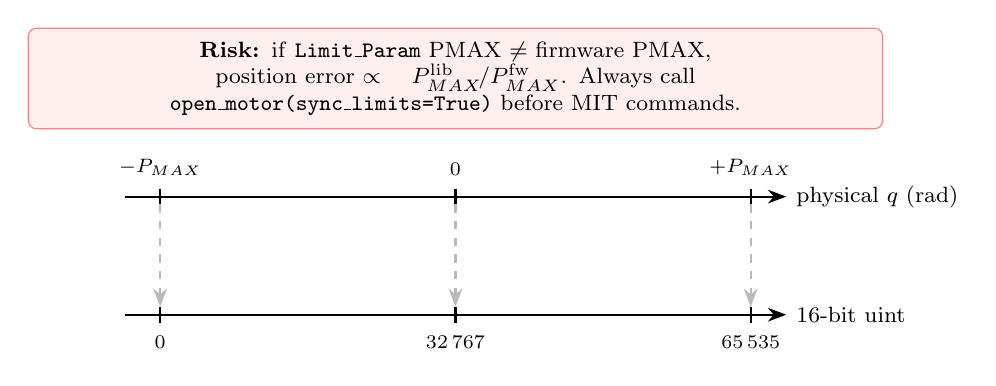
\begin{tikzpicture}[every node/.style={font=\small}, xscale=0.75]
  % Warning banner
  \node[draw=red!50, fill=red!6, rounded corners=3pt, inner sep=5pt,
        text width=10.5cm, align=center, font=\footnotesize]
    at (0, 3.6)
    {\textbf{Risk:} if \texttt{Limit\_Param} PMAX $\neq$ firmware PMAX,
     position error $\propto P_{MAX}^{\text{lib}}\!/P_{MAX}^{\text{fw}}$.
     Always call \texttt{open\_motor(sync\_limits=True)} before MIT commands.};

  % Physical axis
  \draw[-Stealth, thick] (-5.6, 2.1) -- (5.6, 2.1)
    node[right, font=\footnotesize] {physical $q$ (rad)};
  \draw[thick] (-5, 2.2) -- (-5, 2.0);
  \node[above, font=\scriptsize] at (-5, 2.25) {$-P_{MAX}$};
  \draw[thick] (0, 2.2) -- (0, 2.0);
  \node[above, font=\scriptsize] at (0, 2.25) {$0$};
  \draw[thick] (5, 2.2) -- (5, 2.0);
  \node[above, font=\scriptsize] at (5, 2.25) {$+P_{MAX}$};

  % Bit-field axis
  \draw[-Stealth, thick] (-5.6, 0.6) -- (5.6, 0.6)
    node[right, font=\footnotesize] {16-bit uint};
  \draw[thick] (-5, 0.7) -- (-5, 0.5);
  \node[below, font=\scriptsize] at (-5, 0.45) {$0$};
  \draw[thick] (0, 0.7) -- (0, 0.5);
  \node[below, font=\scriptsize] at (0, 0.45) {$32\,767$};
  \draw[thick] (5, 0.7) -- (5, 0.5);
  \node[below, font=\scriptsize] at (5, 0.45) {$65\,535$};

  % Mapping arrows (dashed vertical lines connecting the two axes)
  \draw[-Stealth, dashed, gray!55, line width=0.8pt] (-5, 2.0) -- (-5, 0.7);
  \draw[-Stealth, dashed, gray!55, line width=0.8pt] (0, 2.0) -- (0, 0.7);
  \draw[-Stealth, dashed, gray!55, line width=0.8pt] (5, 2.0) -- (5, 0.7);
\end{tikzpicture}
\caption{Linear quantisation of position for the MIT CAN frame.  Velocity
         uses 12-bit with $\pm V_{MAX}$; torque uses 12-bit with
         $\pm T_{MAX}$.  PMAX / VMAX / TMAX must match firmware exactly.}
\label{fig:quantization}
\end{figure}

\noindent\texttt{open\_motor(sync\_limits=True)} (the default) handles this
automatically:
\begin{lstlisting}
pmax = mc.read_motor_param(motor, DM_variable.PMAX)
vmax = mc.read_motor_param(motor, DM_variable.VMAX)
tmax = mc.read_motor_param(motor, DM_variable.TMAX)
mc.Limit_Param[int(DM_Motor_Type.DM4310)] = [pmax, vmax, tmax]
# For this unit: PMAX=12.5, VMAX=30, TMAX=10
\end{lstlisting}

% ---- Layer 3 -------------------------------------------------------------
\subsection{Layer~3: Runtime zero position}

The output-shaft encoder is absolute single-turn (14-bit), but the
\emph{origin} (what reads as $0\,\mathrm{rad}$) is a writeable firmware
register.  Call \texttt{set\_zero\_position} once after enabling to make
the current physical angle the reference for all subsequent commands.

\begin{figure}[ht]
\centering
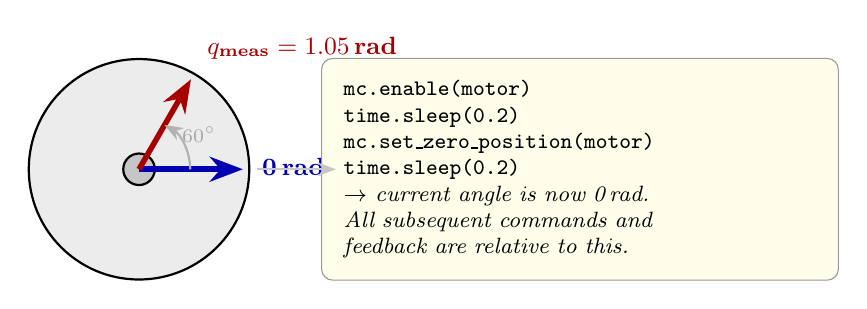
\begin{tikzpicture}[every node/.style={font=\small}]
  % Shaft disc
  \draw[thick, fill=gray!15] (0,0) circle (1.4cm);
  \draw[thick, fill=gray!45] (0,0) circle (0.20cm);

  % Zero-reference arrow (blue, horizontal right)
  \draw[-Stealth, blue!70!black, line width=2pt] (0,0) -- (0:1.32cm);
  \node[right=0.04cm, text=blue!70!black, font=\small\bfseries]
    at (0:1.4cm) {0\,rad\;(\texttt{set\_zero} latched here)};

  % Current measured position (red, at 60 deg)
  \draw[-Stealth, red!65!black, line width=2pt] (0,0) -- (60:1.32cm);
  \node[above right=0.02cm, text=red!65!black, font=\small\bfseries]
    at (60:1.45cm) {$q_{\text{meas}}=1.05\,\text{rad}$};

  % Arc and angle label
  \draw[-Stealth, gray!60, line width=0.8pt] (0:0.65cm) arc (0:60:0.65cm);
  \node[font=\scriptsize, gray!70] at (30:0.88cm) {$60^{\circ}$};

  % Code box to the right
  \node[draw=black!40, fill=yellow!8, rounded corners=4pt, inner sep=8pt,
        text width=6.0cm, align=left, font=\footnotesize]
    at (5.6, 0) {
      \texttt{mc.enable(motor)}\\
      \texttt{time.sleep(0.2)}\\
      \texttt{mc.set\_zero\_position(motor)}\\
      \texttt{time.sleep(0.2)}\\
      \textit{$\to$ current angle is now 0\,rad.}\\
      \textit{All subsequent commands and}\\
      \textit{feedback are relative to this.}
  };
  \draw[-Stealth, gray!45, thick] (1.5, 0) -- (2.5, 0);
\end{tikzpicture}
\caption{\texttt{set\_zero\_position} sends the CAN frame
         \texttt{[0xFF\,\ldots\,0xFE]} which latches the current
         output-shaft encoder reading as $0\,\mathrm{rad}$.  The change
         is volatile unless \texttt{save\_motor\_param()} is called.}
\label{fig:zero-pos}
\end{figure}

\begin{lstlisting}
mc.switchControlMode(motor, Control_Type.MIT)
mc.enable(motor)
time.sleep(0.2)
mc.set_zero_position(motor)    # current angle -> 0 rad (volatile)
time.sleep(0.2)                # firmware needs ~200 ms to commit
# Now all position commands are offsets from this reference
mc.controlMIT(motor, 30.0, 1.0, math.pi/2, 0.0, 0.0)  # +90 deg
\end{lstlisting}

% ---- Verification checklist ----------------------------------------------
\subsection{Verification checklist}
\begin{enumerate}
  \item Power on motor (24\,V).  Connect HDSC USB-to-CAN adapter.
  \item Open Damiao Windows debug tool, click \emph{Read Param}.
        Confirm \texttt{MST\_ID = 0x11} and \texttt{ESC\_ID = 0x01}.
        \textit{If \texttt{MST\_ID = 0x00}: change to \texttt{0x11}, click
        \emph{Write Param}.}
  \item Confirm \texttt{PMAX = 12.5}, \texttt{VMAX = 30},
        \texttt{TMAX = 10}.  Adjust if different.
  \item Run \texttt{python tests/damiao/01\_read\_params.py} -- should print all
        firmware registers without timeout warnings.
  \item Run \texttt{python tests/damiao/03\_pos\_vel\_control.py} -- motor should
        move to $+90^{\circ}$, hold 4\,s, return to $0^{\circ}$.
        Any other angle indicates a PMAX mismatch (Layer~2) or an
        incorrect gear-ratio factor.
\end{enumerate}

% =========================================================================
\section{LeRobot-style Bus Architecture (multi-motor)}
\label{sec:bus}
% =========================================================================

For robots with multiple joints (e.g.\ two Damiao + two CubeMars motors),
a \emph{declarative config + named bus} pattern cleanly separates hardware
wiring from control logic -- following the same contract as
\texttt{lerobot.common.robot\_utils.MotorsBus}.

% ---- Class relationships -------------------------------------------------
\subsection{Class relationships}

\begin{figure}[ht]
\centering
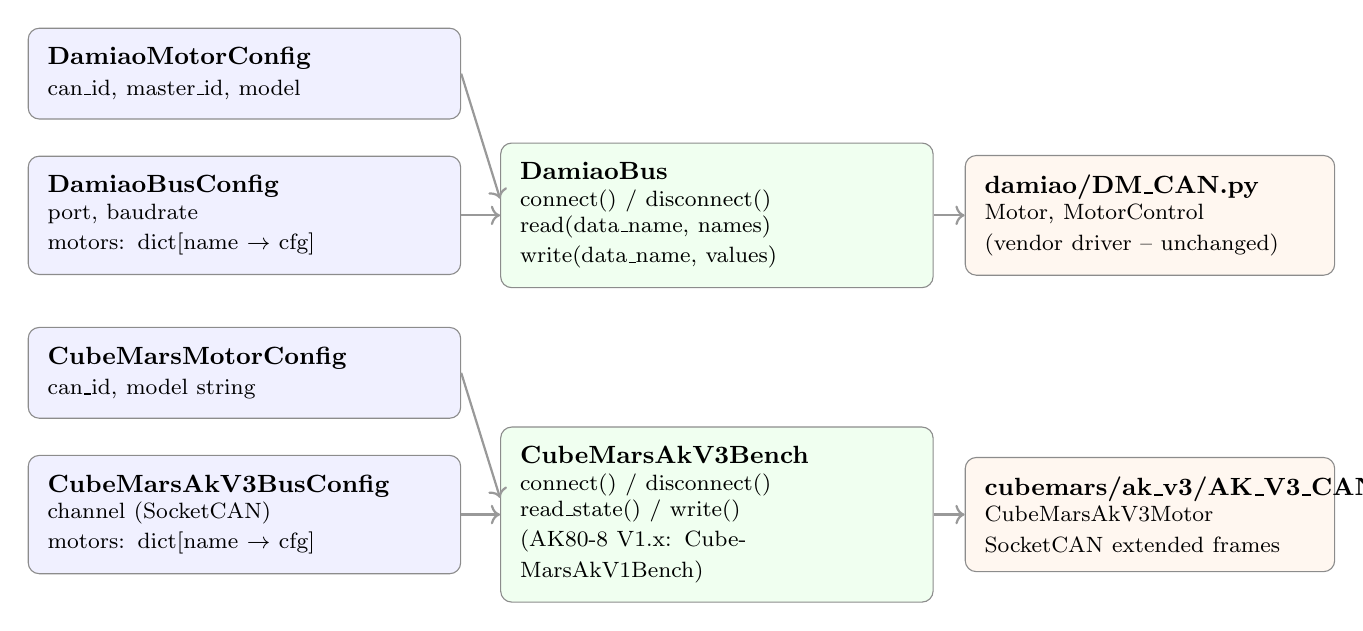
\begin{tikzpicture}[
  every node/.style={font=\small},
  box/.style={draw=black!45, rounded corners=4pt, inner sep=7pt,
              text width=5.0cm, align=left, minimum height=1.0cm},
  cfg/.style={box, fill=blue!6},
  bus/.style={box, fill=green!6},
  drv/.style={box, fill=orange!6, text width=4.2cm},
]
  % Config column
  \node[cfg] (mc) at (-5.5, 1.8)
    {\textbf{DamiaoMotorConfig}\\ \footnotesize can\_id, master\_id, model};
  \node[cfg] (bc) at (-5.5, 0.0)
    {\textbf{DamiaoBusConfig}\\ \footnotesize port, baudrate\\ motors: dict[name $\to$ cfg]};
  \node[cfg] (cc) at (-5.5,-2.0)
    {\textbf{CubeMarsMotorConfig}\\ \footnotesize can\_id, model string};
  \node[cfg] (bcc) at (-5.5,-3.8)
    {\textbf{CubeMarsAkV3BusConfig}\\ \footnotesize channel (SocketCAN)\\ motors: dict[name $\to$ cfg]};

  % Bus column
  \node[bus] (db) at (0.5, 0.0)
    {\textbf{DamiaoBus}\\ \footnotesize connect() / disconnect()\\ read(data\_name, names)\\ write(data\_name, values)};
  \node[bus] (cb) at (0.5,-3.8)
    {\textbf{CubeMarsAkV3Bench}\\ \footnotesize connect() / disconnect()\\ read\_state() / write()\\ (AK80-8 V1.x: CubeMarsAkV1Bench)};

  % Driver / vendor layer
  \node[drv] (dm) at (6.0, 0.0)
    {\textbf{damiao/DM\_CAN.py}\\ \footnotesize Motor, MotorControl\\ (vendor driver -- unchanged)};
  \node[drv] (cu) at (6.0,-3.8)
    {\textbf{cubemars/ak\_v3/AK\_V3\_CAN.py}\\ \footnotesize CubeMarsAkV3Motor\\ SocketCAN extended frames};

  % Arrows: config -> bus
  \draw[->, black!40, thick] (mc.east) -- ([yshift= 6pt]db.west);
  \draw[->, black!40, thick] (bc.east) -- (db.west);
  \draw[->, black!40, thick] (cc.east) -- ([yshift= 6pt]cb.west);
  \draw[->, black!40, thick] (bcc.east) -- (cb.west);
  % Arrows: bus -> driver
  \draw[->, black!40, thick] (db.east)  -- (dm.west);
  \draw[->, black!40, thick] (cb.east)  -- (cu.west);
\end{tikzpicture}
\caption{Separation of concerns.  Config dataclasses hold hardware wiring
         (no driver import needed).  Bus classes wrap vendor drivers behind
         a uniform \texttt{read}/\texttt{write} API.}
\label{fig:bus-arch}
\end{figure}

% ---- Supported data names ------------------------------------------------
\subsection{Supported \texttt{data\_name} values}

\begin{center}\small
\begin{tabular}{llll}
\toprule
Direction & \texttt{data\_name} & Unit & MIT behaviour\\
\midrule
read  & \texttt{position}       & rad     & Decoded from 16-bit POS field\\
read  & \texttt{velocity}       & rad/s   & Decoded from 12-bit VEL field\\
read  & \texttt{torque}         & N$\cdot$m & Decoded from 12-bit TAU field\\
\midrule
write & \texttt{goal\_position} & rad     & controlMIT($K_p$, $K_d$, q, 0, 0)\\
write & \texttt{goal\_velocity} & rad/s   & controlMIT(0, $K_d$, 0, v, 0)\\
write & \texttt{goal\_torque}   & N$\cdot$m & controlMIT(0, 0, 0, 0, $\tau$)\\
write & \texttt{mit\_command}   & rad     & controlMIT($K_p$, $K_d$, q, $\dot{q}$, $\tau_{\text{ff}}$)\\
\bottomrule
\end{tabular}
\end{center}

% ---- Protocol differences ------------------------------------------------
\subsection{Protocol differences: Damiao vs.\ CubeMars}

\begin{center}\small
\begin{tabular}{lll}
\toprule
Property & Damiao DM-J4310-2EC & CubeMars AK-series\\
\midrule
MIT frame & identical 8-byte bit-pack & identical 8-byte bit-pack\\
Feedback CAN ID & \texttt{MST\_ID} (0x11) & \texttt{ESC\_ID} (motor's own ID)\\
Limits source & read from firmware at startup & \texttt{CUBEMARS\_LIMITS} dict\\
Param read/write & yes (read\_motor\_param) & no API available\\
Master ID required & yes (must be 0x11) & no\\
HDSC serial envelope & 30-byte tx, 16-byte rx & same\\
\bottomrule
\end{tabular}
\end{center}

% ---- Complete 2-bus example -------------------------------------------
\subsection{Two-bus example: Damiao joint + CubeMars AK60-6 joint}

\begin{lstlisting}
# robot_arm.py -- Damiao DM-J4310-2EC on UART + AK60-6 V3.0 on CAN
import time, math
from _common import open_bus, open_cubemars_ak_v3_bench, Control_Type

# Damiao joint in MIT position mode; AK60-6 V3.0 joint
with open_bus(mode=Control_Type.MIT, set_zero=True) as dm_bus, \
     open_cubemars_ak_v3_bench(set_zero=True) as ak_bus:

    t0 = time.time()
    while time.time() - t0 < 10.0:          # run for 10 s
        t = time.time() - t0

        # --- Damiao: sinusoidal sweep ----------------------------------
        dm_bus.write("goal_position", {"j1": 0.5 * math.sin(t)},
                     kp=30.0, kd=1.0)
        q_dm, dq_dm, tau_dm = dm_bus.read_state()["j1"]

        # --- AK60-6: mirrored motion at lower stiffness ---------------
        ak_bus.write("goal_position", {"j1": -0.3 * math.sin(t)},
                     kp=60.0, kd=1.5)
        q_ak, dq_ak, ia_ak = ak_bus.read_state()["j1"]

        time.sleep(0.01)      # 100 Hz control loop
\end{lstlisting}

% ---- File layout ---------------------------------------------------------
\subsection{New source files}

\begin{center}\small
\begin{tabular}{ll}
\toprule
File & Purpose\\
\midrule
\texttt{src/motor\_config.py}               & Single source of truth: all hardware configs\\
\texttt{src/\_common.py}                    & Test helpers: \texttt{open\_bus()}, \texttt{open\_cubemars\_ak\_v3\_bench()}, \texttt{open\_cubemars\_ak\_v1\_bench()}\\
\texttt{src/damiao/DM\_CAN.py}              & Vendor driver -- unchanged\\
\texttt{src/damiao/damiao\_bus.py}          & DamiaoBus (wraps DM\_CAN.py)\\
\texttt{src/cubemars/ak\_v3/AK\_V3\_CAN.py} & CubeMars AK60-6 V3.0 CAN driver (\texttt{CubeMarsAkV3Motor})\\
\texttt{src/cubemars/ak\_v3/ak\_v3\_bus.py} & \texttt{CubeMarsAkV3Bench} context manager\\
\texttt{src/cubemars/ak\_v1/AK\_V1\_CAN.py} & CubeMars AK80-8 V1.x CAN driver (\texttt{CubeMarsAkV1Motor})\\
\texttt{src/cubemars/ak\_v1/ak\_v1\_bus.py} & \texttt{CubeMarsAkV1Bench} context manager\\
\bottomrule
\end{tabular}
\end{center}

\section{Hardware summary (from PDF)}
\begin{itemize}
  \item Model: DM--J4310--2EC V1.1, 24\,V geared servo motor with integrated driver.
  \item Gear ratio: 10:1 (output shaft).
  \item Rated / peak torque: 3\,N$\cdot$m / 7\,N$\cdot$m.
  \item Rated speed: 120\,rpm; no-load max: 200\,rpm $\approx 20.94$\,rad/s.
  \item Pole pairs: 14; phase $L=340\,\mu\mathrm{H}$, $R=650\,\mathrm{m}\Omega$.
  \item Encoders: dual 14-bit magnetic, single-turn absolute on output shaft.
  \item CAN: 1\,Mbps, standard frame; UART debug: 921600\,bps.
  \item Recommended supply 15--32\,V; over-current limit $\le 9.8$\,A.
  \item Status LED: green on = enabled; red on = disabled; red blink = fault
        (8 OV, 9 UV, A OC, B MOS over-temp, C coil over-temp, D comm loss, E overload).
\end{itemize}

\section{CAN frame protocol (PDF, section ``Usage'')}
All frames are CAN 2.0A standard, 1\,Mbps. \texttt{ID} below is the motor's CAN
slave ID (\texttt{ESC\_ID}, default 0x01).

\subsection{Feedback frame (Master ID, default 0)}
Always 8 bytes, identical across modes:
\begin{center}\small
\begin{tabular}{lllllllll}
\toprule
D[0] & D[1] & D[2] & D[3] & D[4] & D[5] & D[6] & D[7] \\
\midrule
ID$|$(ERR$\!\ll\!$4) & POS[15:8] & POS[7:0] & VEL[11:4] & VEL[3:0]$|$T[11:8] & T[7:0] & T\_MOS & T\_Rotor \\
\bottomrule
\end{tabular}
\end{center}
\texttt{POS} is 16-bit unsigned mapped linearly to $[-P_{MAX}, +P_{MAX}]$ rad;
\texttt{VEL} and \texttt{T} are 12-bit unsigned mapped to $[-V_{MAX},+V_{MAX}]$
and $[-T_{MAX},+T_{MAX}]$.

\subsection{MIT mode -- CAN ID = ESC\_ID}
8 bytes, bit-packed:
\begin{center}\small
\begin{tabular}{llllllll}
\toprule
D[0] & D[1] & D[2] & D[3] & D[4] & D[5] & D[6] & D[7]\\
\midrule
p[15:8] & p[7:0] & v[11:4] & v[3:0]$|$Kp[11:8] & Kp[7:0] & Kd[11:4] & Kd[3:0]$|$t[11:8] & t[7:0]\\
\bottomrule
\end{tabular}
\end{center}
Ranges: $K_p\in[0,500]$, $K_d\in[0,5]$, $p,v,t$ scaled to motor's
$P_{MAX},V_{MAX},T_{MAX}$. \emph{Do not} set $K_d=0$ when commanding position.

\subsection{Position--Speed mode -- CAN ID = 0x100 + ESC\_ID}
8 bytes, two raw little-endian \texttt{float32}s: bytes 0--3 = \texttt{p\_des}
(rad), bytes 4--7 = \texttt{v\_des} (rad/s, max trapezoidal speed).

\subsection{Speed mode -- CAN ID = 0x200 + ESC\_ID}
4 bytes: little-endian \texttt{float32} \texttt{v\_des} (rad/s).

\subsection{Enable / disable / set-zero special frames}
8-byte command: \texttt{0xFF 0xFF 0xFF 0xFF 0xFF 0xFF 0xFF CMD}
where \texttt{CMD = 0xFC} enable, \texttt{0xFD} disable, \texttt{0xFE} set-zero.

\section{How the Python library maps to the protocol}
File: \texttt{DM\_CAN.py}.
\begin{itemize}
  \item \texttt{controlMIT(motor, kp, kd, q, dq, tau)} -- packs the MIT frame
        exactly as the PDF table; uses \texttt{Limit\_Param[MotorType]} for the
        $\pm P_{MAX}, \pm V_{MAX}, \pm T_{MAX}$ scaling. \textbf{This is the
        critical point}: the scaling \emph{must} match the firmware-side
        $P_{MAX}/V_{MAX}/T_{MAX}$, otherwise the commanded position is silently
        rescaled.
  \item \texttt{control\_Pos\_Vel(motor, p, v)} -- sends \texttt{0x100+ID} with
        two float32s, matches PDF.
  \item \texttt{control\_Vel(motor, v)} -- sends \texttt{0x200+ID} with one
        float32, matches PDF.
  \item \texttt{enable/disable/set\_zero\_position} -- send the
        \texttt{0xFF\dots,0xFC/0xFD/0xFE} special commands.
  \item \texttt{switchControlMode}, \texttt{read/change/save\_motor\_param} --
        UART-side meta commands handled by the USB-to-CAN board.
\end{itemize}

\subsection{\texttt{Limit\_Param} table for DM4310}
\begin{verbatim}
DM4310 :  P_MAX = 12.5 rad,  V_MAX = 30 rad/s,  T_MAX = 10 N.m
\end{verbatim}
There is no dedicated \texttt{DM\_Motor\_Type.DM\_J4310\_2EC} entry. The student's
\texttt{library\_test.py} therefore selects \texttt{DM\_Motor\_Type.DM4310} for a
J-series geared motor, which is the source of the symptom described.

\section{Audit of student's run -- ``it went to another position''}
Symptom: a position command drove the shaft to a different position than
expected.

\subsection{Actual firmware values (read from the unit)}
The Damiao Windows debug tool reports for this specific motor:
\begin{verbatim}
  PMAX = 12.5  rad   VMAX = 30 rad/s   TMAX = 10 N.m
  GR (Gear Ratio)        = 10
  Gear factor (firmware) = 1
  CAN_ID = 0x01     Master_ID = 0x00     <-- WRONG
  Control mode = 1 : MIT
\end{verbatim}
So $P_{MAX}/V_{MAX}/T_{MAX}$ already match the library's
\texttt{DM\_Motor\_Type.DM4310} defaults. The earlier $P_{MAX}$-mismatch
hypothesis does \emph{not} apply here.

\subsection{Real root cause 1 -- the 10:1 gearbox is not compensated}
With \texttt{Gear factor = 1}, the firmware does \textbf{not} divide the
commanded $p\_des$ by the gear ratio. CAN-side commands are interpreted on the
\emph{rotor} side, so a command of $q=8$\,rad on the rotor produces only
$8/10 = 0.8$\,rad on the output shaft. To move the output shaft by
$\theta$\,rad, send $10\theta$\,rad on CAN.

\subsection{Real root cause 2 -- Master ID = 0x00}
The firmware sends feedback with \texttt{Master\_ID} as the CAN ID. The Python
\texttt{Motor} object filters incoming frames against the \texttt{MasterID}
passed at construction (the example uses \texttt{0x11}). With firmware
set to \texttt{0x00}, the library's \texttt{recv()} drops the feedback and
\texttt{getPosition()/getVelocity()/getTorque()} stay stale. Seeed and the
Damiao docs both warn: \emph{do not leave Master\,ID at 0}. Set it to
\texttt{CAN\_ID + 0x10} via the debug tool, then \emph{Write Param}.

\subsection{Earlier general note -- $P_{MAX}$ mismatch on other firmware}
Some J-series units ship with a smaller $P_{MAX}$ (e.g.\ $\pi$\,rad). For
those, the 16-bit POS field is decoded as
\[
q_{\text{actual}} = \frac{\text{POS}}{2^{16}-1}\,2P_{MAX}^{\text{firmware}} - P_{MAX}^{\text{firmware}},
\]
so a Python-side encode using $P_{MAX}^{\text{lib}}=12.5$ silently rescales
the command. Always read \texttt{PMAX, VMAX, TMAX} on start-up and overwrite
\texttt{Limit\_Param[DM4310]}. The helper in \texttt{tests/\_common.py} does
this automatically:
\begin{lstlisting}
pmax = mc.read_motor_param(motor, DM_variable.PMAX)
vmax = mc.read_motor_param(motor, DM_variable.VMAX)
tmax = mc.read_motor_param(motor, DM_variable.TMAX)
mc.Limit_Param[int(DM_Motor_Type.DM4310)] = [pmax, vmax, tmax]
\end{lstlisting}

\subsection{Secondary issues found}
\begin{enumerate}
  \item \textbf{\texttt{time.sleep} bug (now fixed)} -- \texttt{DM\_CAN.py}
        previously had \texttt{from time import sleep} but called
        \texttt{time.sleep(0.001)} inside \texttt{control\_Pos\_Vel}, which
        raises \texttt{NameError: name 'time' is not defined} the first time
        position--speed mode is used. Patched by adding \texttt{import time}.
  \item \textbf{Position--Speed v\_des} is the trapezoidal cruise speed; if it
        is left at 0 the motor will not move. The student's loop uses
        \texttt{control\_Pos\_Vel(Motor1, q*8, 30)} which is fine.
  \item \textbf{$K_d = 0$ in MIT position mode} causes oscillation/loss of
        control (PDF note). When using \texttt{controlMIT} for positioning,
        keep $K_d>0$ (e.g.\ 0.5--2 for J4310).
  \item \textbf{Communication-loss timeout}: if no CAN frame is received within
        the configured \texttt{TIMEOUT} the driver auto-disables. Send at least
        one command per timeout period.
  \item \textbf{Bit-shift width on \texttt{numpy.uint16}} -- \texttt{q\_uint
        >> 8} is performed on a \texttt{numpy.uint16}; this is correct but a
        plain \texttt{int} cast is safer if the type ever changes.
\end{enumerate}

\section{Recommended quick-start in MIT mode (DM--J4310--2EC)}
\begin{lstlisting}
m = Motor(DM_Motor_Type.DM4310, SlaveID=0x01, MasterID=0x11)
mc = MotorControl(serial.Serial('/dev/ttyACM0', 921600, timeout=0.5))
mc.addMotor(m)

# Sync library limits with firmware-stored ones (CRITICAL for J-series)
pmax = mc.read_motor_param(m, DM_variable.PMAX)
vmax = mc.read_motor_param(m, DM_variable.VMAX)
tmax = mc.read_motor_param(m, DM_variable.TMAX)
mc.Limit_Param[int(DM_Motor_Type.DM4310)] = [pmax, vmax, tmax]

mc.switchControlMode(m, Control_Type.MIT)
mc.enable(m)
mc.set_zero_position(m)            # define current pose as 0 rad
mc.controlMIT(m, kp=30, kd=1.0, q=1.57, dq=0, tau=0)  # 90 deg
\end{lstlisting}

\section{Recommended quick-start in Position--Speed mode}
\begin{lstlisting}
mc.switchControlMode(m, Control_Type.POS_VEL)
mc.enable(m)
mc.control_Pos_Vel(m, P_desired=1.57, V_desired=5.0)  # rad, rad/s
\end{lstlisting}

% =========================================================================
\section{Control modes -- full reference with Python examples}
% =========================================================================
All commanded and feedback values are in \textbf{output-shaft units}
(rad, rad/s, N$\cdot$m).  The 10:1 gearbox is transparent to the user.

\subsection{Position-Speed mode (\texttt{CAN\_ID = 0x100 + ESC\_ID})}
\textbf{What it does.}
Three-loop cascade (position $\to$ speed $\to$ current).
\texttt{p\_des} is the target position; \texttt{v\_des} caps the trapezoidal
cruise speed.  The motor generates its own acceleration/deceleration profile.

\textbf{Best for:} deterministic point-to-point moves, robot joint positioning,
pick-and-place.

\begin{lstlisting}
# 03_pos_vel_control.py  -- move to 90 deg and return
import math, time
from _common import open_bus
from DM_CAN import Control_Type

with open_bus(mode=Control_Type.POS_VEL, set_zero=True) as bus:
    for _ in range(400):
        bus.write("goal_pos_vel", {"j1": math.pi/2}, dq_des=5.0)
        time.sleep(0.01)
    for _ in range(400):
        bus.write("goal_pos_vel", {"j1": 0.0}, dq_des=5.0)
        time.sleep(0.01)
\end{lstlisting}

\noindent\textbf{Key parameters:}
\begin{itemize}
  \item \texttt{Acc / Dec} (set in firmware): shape the ramp; increase if
        oscillation appears at the end of movement.
  \item \texttt{v\_des = 0} prevents movement -- always set a non-zero cruise speed.
\end{itemize}

% -------------------------------------------------------------------------
\subsection{Speed mode (\texttt{CAN\_ID = 0x200 + ESC\_ID})}
\textbf{What it does.}
Single-loop velocity control.  The motor maintains the commanded speed.
Position is ignored.

\textbf{Best for:} continuous rotation, conveyor-like tasks, proportional
joystick control.

\begin{lstlisting}
# 04_speed_control.py  -- spin +5 rad/s then reverse
import time
from _common import open_bus
from DM_CAN import Control_Type

with open_bus(mode=Control_Type.VEL) as bus:
    for vel in [5.0, 0.0, -5.0, 0.0]:
        for _ in range(200):
            bus.write("goal_speed", {"j1": vel})
            time.sleep(0.01)
\end{lstlisting}

% -------------------------------------------------------------------------
\subsection{MIT mode (\texttt{CAN\_ID = ESC\_ID}) -- three sub-modes}
The MIT frame sends five scalars in 8 bytes.  The motor computes:
\[
\tau_{\text{ref}} = K_p\bigl(q_{\text{des}}-q_{\text{meas}}\bigr)
                  + K_d\bigl(\dot{q}_{\text{des}}-\dot{q}_{\text{meas}}\bigr)
                  + \tau_{\text{ff}}
\]
By choosing which parameters are non-zero you get three distinct sub-modes.

\subsubsection{MIT Position control ($K_p>0$, $K_d>0$)}
\textbf{Best for:} tight position hold, fast response, back-drivability tuning.

\begin{lstlisting}
# 05_mit_position.py
import math, time
from _common import open_bus

KP, KD = 30.0, 1.0     # Kp in [0,500], Kd in [0,5]
with open_bus(set_zero=True) as bus:
    for target in [math.pi/2, 0.0, -math.pi/4, 0.0]:
        for _ in range(300):
            bus.write("goal_position", {"j1": target}, kp=KP, kd=KD)
            time.sleep(0.01)
\end{lstlisting}

\noindent\textbf{Tuning:}
\begin{itemize}
  \item Increase $K_p$ for stiffer hold; decrease if the joint vibrates.
  \item Increase $K_d$ to damp oscillations; too high feels sluggish.
  \item \textbf{Never set $K_d = 0$ when commanding position} -- see PDF note.
\end{itemize}

\subsubsection{MIT Velocity control ($K_p=0$, $K_d>0$)}
\textbf{Best for:} smooth continuous rotation where precise position is not needed.

\begin{lstlisting}
# 06_mit_velocity.py
import time
from _common import open_bus

KD = 1.0
with open_bus() as bus:
    for dq in [3.0, 0.0, -3.0, 0.0]:
        for _ in range(200):
            bus.write("goal_velocity", {"j1": dq}, kd=KD)
            time.sleep(0.01)
\end{lstlisting}

\subsubsection{MIT Torque control ($K_p=0$, $K_d=0$, $\tau_{\text{ff}}\neq0$)}
\textbf{Best for:} force/impedance control, compliant tasks.
Position and velocity are fully uncontrolled -- the motor will accelerate
if unloaded.  Always use a mechanical stop or external safety check.

\begin{lstlisting}
# 07_mit_torque.py
import time
from _common import open_bus

TAU = 0.5   # N.m -- keep small for unloaded tests
with open_bus() as bus:
    t0 = time.time()
    while time.time() - t0 < 1.5:
        bus.write("goal_torque", {"j1": TAU})
        time.sleep(0.01)
    # Damp to stop before disable
    for _ in range(100):
        bus.write("goal_velocity", {"j1": 0.0}, kd=1.0)
        time.sleep(0.01)
\end{lstlisting}

\subsection{Mode comparison}
\begin{center}\small
\begin{tabular}{lllll}
\toprule
Mode & CAN ID & Position? & Speed? & Tuning\\
\midrule
Position-Speed & \texttt{0x100+ID} & \checkmark & via ramp & None\\
Speed          & \texttt{0x200+ID} & --         & \checkmark & None\\
MIT Position   & \texttt{ID}       & \checkmark & damped & $K_p$, $K_d$\\
MIT Velocity   & \texttt{ID}       & --         & \checkmark & $K_d$\\
MIT Torque     & \texttt{ID}       & --         & --         & --\\
\bottomrule
\end{tabular}
\end{center}

% =========================================================================
\section{Impedance control and kinesthetic teaching}
\label{sec:impedance}
% =========================================================================
\subsection{Concept}
Impedance control makes the joint behave like a \emph{virtual spring-damper}:
\[
\tau_{\text{cmd}} = K_p(q_{\text{des}}-q_{\text{meas}}) + K_d(\dot{q}_{\text{des}}-\dot{q}_{\text{meas}}) + \tau_{\text{ff}}
\]
By lowering $K_p$ and $K_d$, the joint becomes \emph{compliant}: an external
force (your hand) can move it, and the motor applies only a gentle restoring
force.  This is the mechanism behind \textbf{kinesthetic teaching /
teleoperation recording} used in imitation learning (e.g.\ ACT, DiffPolicy,
UMI).

\subsection{Physical interpretation of $K_p$ and $K_d$}
\begin{itemize}
  \item $K_p$ (N$\cdot$rad$^{-1}$): virtual spring stiffness.  $K_p = 0$
        means the joint is completely free.
        $K_p = 30$ -- light spring, easy to push.
        $K_p = 300$ -- stiff, hard to backdrive.
  \item $K_d$ (N$\cdot$s$\cdot$rad$^{-1}$): virtual damping.  Low $K_d$
        ($< 0.2$) feels frictionless but may vibrate.
        $K_d \approx 0.5$--$1.0$ feels smooth.
\end{itemize}

\subsection{Recipe: ``gravity-compensation + hand guiding''}

\begin{enumerate}
  \item Switch to MIT mode.  Enable the motor.
  \item Set $q_{\text{des}}=q_{\text{meas}}$ (current position) so the spring
        force is initially zero.
  \item Set low $K_p$ (e.g.\ 5--15) and low $K_d$ (e.g.\ 0.3--0.8).
  \item Add a $\tau_{\text{ff}}$ term that compensates gravity if the joint
        carries a load.
  \item Record $q_{\text{meas}}$ at each timestep -- this is your demonstration.
\end{enumerate}

\begin{lstlisting}
"""08_kinesthetic_record.py -- move the motor by hand and record trajectory."""
import time, csv
from _common import open_bus

KP, KD = 5.0, 0.5
RECORD_HZ = 100

trajectory = []
with open_bus() as bus:
    bus.refresh()                         # prime state cache
    q_hold = bus.read_state()["j1"][0]    # start at current position
    print("Move the motor by hand. Press Ctrl+C to finish.")
    t0 = time.time()
    try:
        while True:
            q, dq, tau = bus.read_state()["j1"]
            t = time.time() - t0
            q_hold = q
            bus.write("mit_command", {"j1": q_hold}, kp=KP, kd=KD)
            trajectory.append([t, q, dq, tau])
            time.sleep(1.0 / RECORD_HZ)
    except KeyboardInterrupt:
        print(f"\nRecorded {len(trajectory)} samples.")

with open("demo_trajectory.csv", "w", newline="") as f:
    csv.writer(f).writerows([["t", "q", "dq", "tau"]] + trajectory)
print("Saved demo_trajectory.csv")
\end{lstlisting}

\noindent This script is provided in the repo as
\texttt{tests/damiao/08\_kinesthetic\_record.py}.

\subsection{Spring-return to origin (\texttt{tests/damiao/10\_impedance\_spring\_return.py})}
A companion script that uses MIT position mode with moderate stiffness to pull
the joint back to zero after a demonstration:
\begin{lstlisting}
# 10_impedance_spring_return.py
import time
from _common import open_bus

ORIGIN, KP, KD = 0.0, 20.0, 0.8
with open_bus(set_zero=True) as bus:
    print("Returning to origin. Press Ctrl+C to stop.")
    try:
        while True:
            q, dq, tau = bus.read_state()["j1"]
            bus.write("goal_position", {"j1": ORIGIN}, kp=KP, kd=KD)
            time.sleep(0.01)
    except KeyboardInterrupt:
        pass
\end{lstlisting}

\subsection{Replaying a demonstration (imitation learning data collection)}
After recording, load the CSV and replay:
\begin{lstlisting}
# 09_replay_trajectory.py
import csv, time
from _common import open_bus

with open_bus() as bus:
    with open("demo_trajectory.csv") as f:
        rows = list(csv.DictReader(f))
    dt = float(rows[1]["t"]) - float(rows[0]["t"])
    for row in rows:
        q = float(row["q"])
        bus.write("goal_position", {"j1": q}, kp=30.0, kd=1.0)
        time.sleep(dt)
\end{lstlisting}

\subsection{Parameter guidelines for different tasks}
\begin{center}\small
\begin{tabular}{llll}
\toprule
Task & $K_p$ & $K_d$ & Notes\\
\midrule
Kinesthetic teaching (hand guiding) & 0--10 & 0.3--0.8 & Soft; operator moves joint\\
Gravity compensation only           & 0     & 0.5--1.0 & Float; $\tau_{\text{ff}}$ holds weight\\
Impedance tracking (light spring)   & 10--30 & 0.5--1.5 & Pushable but returns\\
Stiff position hold                 & 100--300 & 1--3  & Hard to backdrive\\
Replay / execution                  & 30--80 & 1--2  & Balance accuracy vs compliance\\
\bottomrule
\end{tabular}
\end{center}

\subsection{Safety considerations}
\begin{itemize}
  \item During hand guiding, always have an emergency-stop key (see
        \texttt{Ctrl+C} handler) or a hardware cut-off on the 24\,V rail.
  \item $K_p=0, K_d=0$ (pure torque) will accelerate if $\tau_{\text{ff}}\neq0$ --
        only use with mechanical limits or while holding the link.
  \item Keep communication rate $\ge 100$\,Hz.  If the control loop drops
        below $\sim$50\,Hz the apparent damping decreases and oscillations
        may appear.
  \item The motor's overcurrent limit is 9.8\,A; do not command torques
        that exceed peak torque (7\,N$\cdot$m at the output shaft).
\end{itemize}

% =========================================================================
\section{Useful references in this repo}
% =========================================================================
\begin{itemize}
  \item \texttt{docs/DM-J4310-en.pdf} -- the manual that this note summarises.
  \item \texttt{src/damiao/DM\_CAN.py} -- vendor driver (unchanged). Mirror at
        \texttt{old/motor-control-routine/Python例程/u2can/DM\_CAN.py}.
  \item \texttt{src/motor\_config.py} -- single source of truth for hardware
        wiring (\texttt{DamiaoMotorConfig}, \texttt{DamiaoBusConfig},
        \texttt{CubeMarsMotorConfig}, \texttt{CubeMarsAkV3BusConfig},
        \texttt{CubeMarsAkV1BusConfig},
        \texttt{DEFAULT\_BENCH\_CONFIG}, \texttt{DEFAULT\_AK60\_6\_BENCH\_CONFIG},
        \texttt{DEFAULT\_AK80\_8\_BENCH\_CONFIG}).
  \item \texttt{src/damiao/damiao\_bus.py} -- LeRobot-style \texttt{DamiaoBus} wrapper.
  \item \texttt{src/cubemars/ak\_v3/ak\_v3\_bus.py} -- \texttt{CubeMarsAkV3Bench}
        for CubeMars AK60-6 V3.0 (same bus contract as \texttt{DamiaoBus}).
  \item \texttt{src/cubemars/ak\_v1/ak\_v1\_bus.py} -- \texttt{CubeMarsAkV1Bench}
        for CubeMars AK80-8 V1.x.
  \item \texttt{src/\_common.py} -- test helpers: \texttt{open\_bus()} context
        manager (tests 03--10), \texttt{open\_motor()} + \texttt{safe\_disable\_close()}
        (legacy tests 01--02 only).
  \item \texttt{tests/} -- numbered test scripts 01--10 (see
        Table~\ref{tab:test-scripts}).
  \item \texttt{motor-control-routine/} -- C, C\#, MATLAB, ROS, STM32 examples.
  \item \texttt{old/} -- archived root-level files (not active).
\end{itemize}

\begin{table}[ht]\centering\small
\caption{Test scripts overview}\label{tab:test-scripts}
\begin{tabular}{lll}
\toprule
File & Mode & Purpose\\
\midrule
\texttt{01\_read\_params.py}  & UART & Dump all firmware params\\
\texttt{02\_write\_params.py} & UART & Edit one param with confirmation\\
\texttt{03\_pos\_vel\_control.py} & Pos-Speed & Point-to-point move\\
\texttt{04\_speed\_control.py}    & Speed     & Constant speed spin\\
\texttt{05\_mit\_position.py}     & MIT Pos   & Kp/Kd position hold\\
\texttt{06\_mit\_velocity.py}     & MIT Vel   & Velocity tracking\\
\texttt{07\_mit\_torque.py}       & MIT Torque & Open-loop torque\\
\texttt{08\_kinesthetic\_record.py}    & MIT & Hand guiding + CSV record\\
\texttt{09\_replay\_trajectory.py}     & MIT & Replay recorded demo\\
\texttt{10\_impedance\_spring\_return.py} & MIT & Spring return to origin\\
\texttt{11\_cable\_wind\_to\_tension.py} & MIT Torque & Cable slack removal; winds until taut\\
\bottomrule
\end{tabular}
\end{table}

\noindent\textbf{Note on test 11.}  See the companion document
\texttt{dm\_j4310\_low\_tension\_notes.tex} (and its compiled PDF) for the
full theory, parameter selection guide, and state-machine description
behind \texttt{11\_cable\_wind\_to\_tension.py}.

\end{document}
